\documentclass{beamer}
\renewcommand\thesection{\arabic{section}}
\newcommand{\myfont}{\rmfamily\normalsize\upshape\mdseries}
\newcommand{\degree}{^\circ}
\title{\sffamily Review I(Slides 20 - 69)}
\subtitle{\textbf{Logics,Sets,Numbers}\\``Without them, mathematics will fall apart... "}
\institute[UM-SJTU JI]{University of Michigan-Shanghai Jiao Tong University Joint Institute}
\author{Kulu}
\usepackage{graphicx}
\usepackage{picinpar}
\usepackage{indentfirst}
\usepackage{chemformula}
\usepackage{geometry}
\usepackage{subfigure}
\usepackage{appendix}
\usepackage{amsfonts,amsmath,amssymb}
\usepackage{enumerate}
\usepackage{float}
\usepackage{geometry}
\usepackage{latexsym}
\usepackage{listings}
\usepackage{multicol,multirow,multido}
\usepackage{tabularx}
\usepackage{ulem}
\usepackage{tikz}
\usepackage{xcolor}
\usepackage{cite}
\usepackage{setspace}
\usepackage{hyperref}
\usepackage{textpos}
\usepackage{booktabs}

\usetheme[dove]{Boadilla}
\usecolortheme{dolphin}
\useoutertheme{miniframes}
\begin{document}
\usebackgroundtemplate{\tikz\node[opacity=0.1]{
        \centerline{
\includegraphics[
                height=\paperheight]{kulu.jpg}}
    };}
\begin{titlepage}
    \begin{center}
        VV186 - Honors Mathmatics II
    \end{center}
\end{titlepage}
\myfont
\section{Introduction}
\begin{frame}
    \frametitle{About Me}
    Schedule
    \begin{itemize}
        \item RC: Thursday 16:00 - 17:40
        \item OH: Thursday 17:40 - 19:40
    \end{itemize}
    Any questions or advice ? Please contact me !
    \begin{itemize}
        \item Email: heyinong@sjtu.edu.cn
    \end{itemize}
    Something more about me:
    \begin{itemize}
        \item Name: Heyinong
        \item Nickname: Kulu (A long story behind)
        \item JI SSTIA Minister
        \item Love music, love piano. Enjoy everything a normal student in University may enjoy.
    \end{itemize}

\end{frame}


\section{Logics}
\begin{frame}
    \frametitle{Statement}
    \small Frequently asked questions: What's the difference between statement and a statement frame ? What's a predicate ?
    First, recall the definition...
    \vspace*{0.5em}
    \begin{itemize}
        \item statement
              \begin{itemize}
                  \item true statement
                  \item false statement
              \end{itemize}
        \item statement structure
              \begin{itemize}
                  \item quantifier
                  \item statement frame/predicate
                  \item specific value
              \end{itemize}
    \end{itemize}
    \vspace*{1em}
    \myfont
    Easy... but be careful! \\
    \textcolor{red}{Definitions? Examples? Notations?}
\end{frame}

\begin{frame}
    \frametitle{Logical Operation}
    Question: Are you familiar with their truth tables and notations?
    \begin{table}
        \centering
        \resizebox{6cm}{!}{
            \begin{tabular}{c|cc|c}
                \hline \hline
                Type                     & \multicolumn{2}{c}{ Logical Operation } & Priority        \\
                \hline
                unary                    & $\neg$                                  & Negation    & 1 \\ \hline
                                         & $\wedge$                                & Conjunction & 2 \\
                                         & $\vee$                                  & Disjunction & 3 \\
                                         & $\Rightarrow$                           & Implication & 4 \\
                \multirow{-4}{*}{binary} & $\Leftrightarrow$                       & Equivalence & 5 \\
                \hline \hline
            \end{tabular}
        }
    \end{table}
    \begin{itemize}
        \item  compound statement
              \begin{itemize}
                  \item \itshape tautology
                  \item contradiction
                  \item contingency
              \end{itemize}
    \end{itemize}
\end{frame}

\begin{frame}
    \frametitle{$Q\&A$: How to interpret implication : $A\Rightarrow B$ ?}
    \begin{itemize}
        \item A implies B / if A then B / A only if B
        \item $A\Rightarrow B \equiv \neg(A\wedge \neg B) \equiv \neg A\vee B$ (Proof by Contradiction)
        \item vacuous truth
              \begin{itemize}
                  \item pink elephants could fly!
                  \item more examples?
                  \item A vacuous truth may have the form similar to :
                        \begin{itemize}
                            \item $A\Rightarrow B$,where A is false
                            \item $\forall x, A(x)\Rightarrow B(x),$ where $\forall x, \neg A(x)$
                            \item $\forall x\in A, B(x)$, where A is an empty set.
                        \end{itemize}
              \end{itemize}
    \end{itemize}
\end{frame}

\begin{frame}
    \frametitle{$Q\&A$: What's the difference between \textbf{equivalence($\Leftrightarrow$)} and \textbf{logically equivalent($\equiv$)}?}
    \begin{itemize}
        \item equivalence ($\Leftrightarrow$) is just one of the binary logical operators. It inputs two statements and returns a single statement. It can be $\textbf{either true or false}$.

              Conventionally, we can just understand it as "if and only if".
        \item logically equivalent ($\equiv$) tells the relationship between two statements. $A\equiv B$ if they have same truth value for all possible combinations of truth values assigned to all variables appearing in A and B. i.e. $A\Leftrightarrow B$ is a tautology.
    \end{itemize}
\end{frame}

\begin{frame}
    \frametitle{Truth Table}
    How to prove logically equivalent? Use truth table !
    \begin{itemize}
        \item How to use a truth table?
              \begin{itemize}
                  \item Understand the problem is about
                  \item Cover all the possible situations
                  \item e.g. Prove \textbf{\itshape de Morgen rules} for statements and sets:\\
                        \vspace*{1em}
                        \* \* \* \*
                        $\neg(A\wedge B)\equiv(\neg A)\vee(\neg B)$
                        \* \* \* \* \* \* \* \*
                        $\neg(A\wedge B)\equiv(\neg A)\vee(\neg B)$

                        \vspace*{1em}
                        \* \* \* \*
                        $(A\cap B)^{c}=A^{c}\cup B^{c}$
                        \* \* \* \* \* \* \* \*\*\*
                        $(A\cup B)^{c}=A^{c}\cap B^{c}$

                        \vspace*{1em}

                        How to prove a logical equivalence? Truth table !

                        How to prove two sets P=Q? (I)$P\subset Q$ (II)$Q\subset P$

                        \vspace*{1em}
                        Observation: Sets and statements are similar.

                        Why are \textbf{\itshape de Morgen rules} so important?
                        \begin{itemize}
                            \item switch between $\vee$ and $\wedge$ using $\neg$. (Frequent in Exercises)
                        \end{itemize}
              \end{itemize}
    \end{itemize}
    \vspace*{5em}
\end{frame}

\begin{frame}
\end{frame}


\begin{frame}
    \frametitle{Relations}
    Those two relations are useful for our mindset when facing an exercise.
    \begin{itemize}
        \item Proof by Contradiction
              \begin{equation*}
                  (A \Rightarrow B) \equiv \neg (A \wedge \neg B)
              \end{equation*}
              We just have one condition A at first, through proof by contradiction, we have two conditions: A and B. So you have one more condition to play with.
        \item Proof by Contraposition
              \begin{equation*}
                  (A\Rightarrow B) \equiv (\neg B \Rightarrow \neg A)
              \end{equation*}
              Through contraposition, we don't get addition conditions, but the mindset is changed. If it's easier to use B than A, you can try thinking about contraposition.
    \end{itemize}
\end{frame}

\begin{frame}
    \frametitle{An exercise from assignment}
    \begin{figure}[htbp]
        \centering
        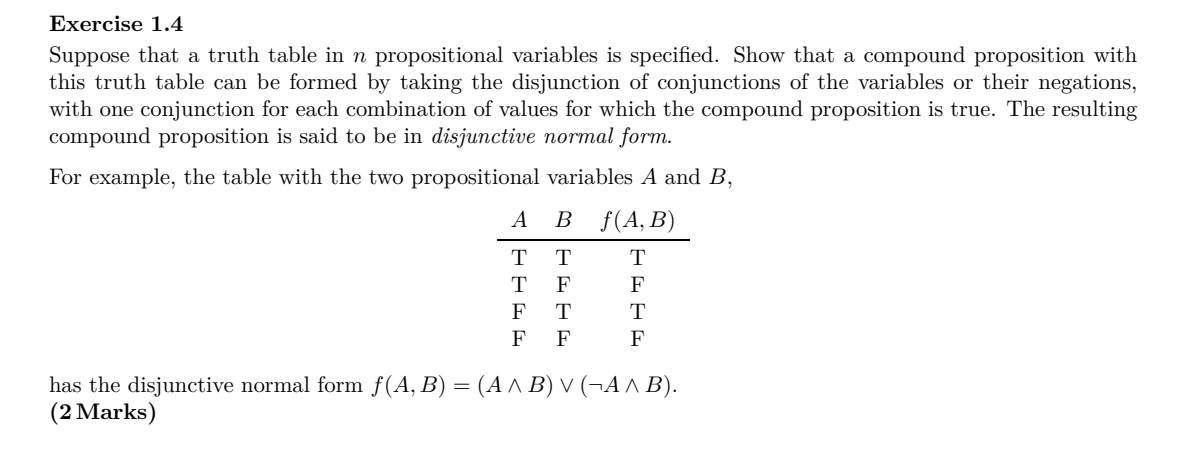
\includegraphics[width=12cm]{exercise1.png}
    \end{figure}
\end{frame}

\begin{frame}
    \frametitle{An example to illustrate DNF and CNF}
    \begin{figure}[htbp]
        \centering
        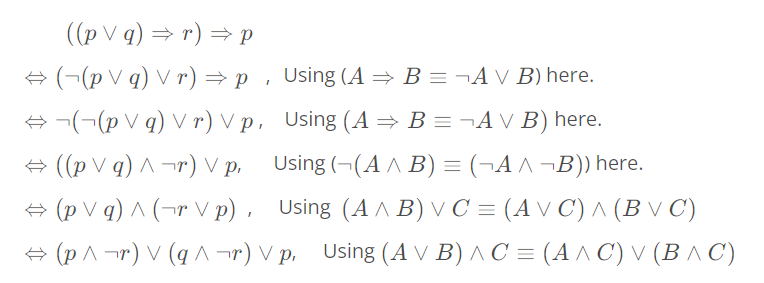
\includegraphics[width=12cm]{example1.png}
    \end{figure}
\end{frame}

\begin{frame}
\end{frame}

\begin{frame}
    \frametitle{DNF and CNF}
    \begin{itemize}
        \item Definition for DNF and CNF
              \begin{itemize}
                  \item Disjunctive Normal Form (DNF): A disjunction of one or more conjunctions of one or more variables or their negations.
                  \item Conjunctive Normal Form (CNF): A conjunction of one or more disjunctions of one or more variables or their negations.
              \end{itemize}
              \vspace*{1em}
        \item Principal Disjunctive Normal Form $\&$ Principal Conjunctive Normal Form
    \end{itemize}
\end{frame}

\begin{frame}
    \frametitle{Logical Quantifiers}
    \begin{table}
        \centering
        \resizebox{12cm}{!}{%
            \begin{tabular}{ccc}
                \toprule
                \multicolumn{3}{c}{Logical Quantifiers}                                                                \\
                \midrule
                Sign                           & Type               & Interpretation                                   \\
                \hline
                $\forall$                      & universal          & for any; for all                                 \\
                $\exists$                      & existential        & there exist; there is some                       \\
                $\forall \dots \forall \dots $ & nesting quantifier & for all \dots for all \dots                      \\
                $\exists \dots \exists \dots $ & nesting quantifier & there exists \dots (such that) there exist \dots \\
                $\forall \dots \exists \dots $ & nesting quantifier & for any \dots, there exists \dots                \\
                $\exists \dots \forall \dots $ & nesting quantifier & there exists \dots (such that) for any \dots     \\
                \dots                          & \dots              & \dots                                            \\
                \bottomrule
            \end{tabular}%
        }
    \end{table}
    \vspace*{1em}
    \begin{itemize}
        \item Hanging Quantifier, be careful with the order.
    \end{itemize}
\end{frame}

\begin{frame}
    \frametitle{Order Matters when quantifiers are different}
    \begin{figure}[htbp]
        \centering
        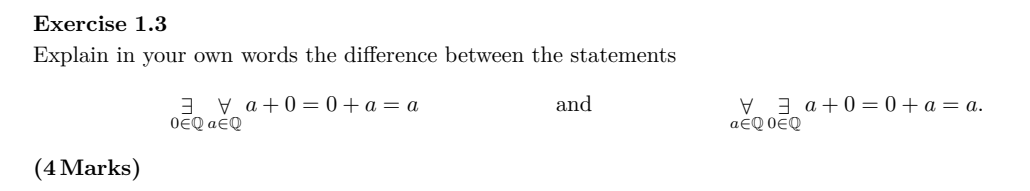
\includegraphics[width=12cm]{exercise2.png}
    \end{figure}
\end{frame}

\begin{frame}
    \frametitle{Negation for logical quantifiers}
    Use quantifiers to rewrite the following definition of covergence:
    \par \vspace{2em} \hspace{1em} Let $(a_n)_{n\in \mathbb{N}}$ be a real sequence. If for some fixed $a \in \mathbb{R}$,
    for any $\varepsilon>0$, there is an $N\in \mathbb{N}$, such that for all $n>N$, $|a_n-a|<\varepsilon$,\\ then we
    say $(a_n)$ converges to $a$.\\
    \vspace{1.5em}
    What's the negation of this statement?

    \vspace{1.5em}
    Steps to write out a negation of a statement:

    (I) Transfer every $\forall$ to $\exists$ and transfer every $\exists$ to $\forall$

    (II) Take the negation of predicates
\end{frame}


\begin{frame}
\end{frame}

\begin{frame}
    \frametitle{Functionally Complete}
    \begin{figure}[htbp]
        \centering
        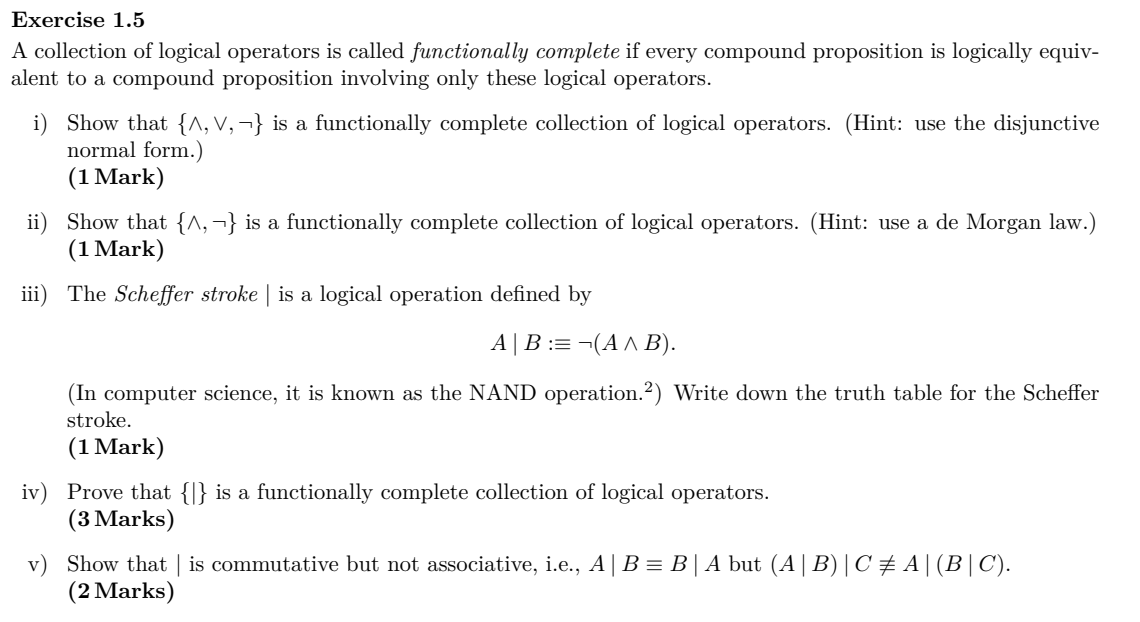
\includegraphics[width=12cm]{exercise3.png}
    \end{figure}
\end{frame}

\begin{frame}
\end{frame}

\begin{frame}
    \frametitle{Optional Questions}
    1. How to show that $\{\wedge ,\vee\}$ is \textbf{NOT} functionally complete?

    \vspace{1em}
    2. Scheffer stroke (|) is also called "NAND". Similarly, Peirce arrow ($\downarrow$) is called "NOR".
    $P \downarrow Q$ is true iff: P and Q are both false.

    Please use "$\downarrow"$ only to construct the statement $P\Rightarrow Q$.
\end{frame}

\section{Sets}
\begin{frame}
    \frametitle{Sets}
    \begin{itemize}
        \item What is a set?
        \item How to interpret a set $\{1,2,3,4,3,4\}$? The elments can be the same ?
        \item Common Type of Set
              \begin{itemize}
                  \item Empty set: $\emptyset := \{x:x\neq x\}$
                  \item Total set
                  \item Subset
                  \item Proper subset
                  \item Power set(finite)

                        Question: What's the power set for $\emptyset$ and for $\{\emptyset\}$?
              \end{itemize}
        \item Cardinality(finite)
    \end{itemize}
    \vspace*{1em}
    \begin{block}{
            Quick check:}
        \hspace{1em}
        Let $X=\{x:P(x)\}.$  Is $P(x)$ a statement?
    \end{block}
\end{frame}
\begin{frame}
    \frametitle{Operations on Sets}
    Let
    \begin{equation*}
        A:=\{1,2\} \quad B:=\{2,3\} \quad M:=\{1,2,3,4,5\}
    \end{equation*}
    Please recall the operations and calculate !
    \begin{table}
        \centering
        \resizebox{6cm}{!}{%
            \begin{tabular}{ccc}
                \toprule
                \multicolumn{3}{c}{Set Operations}    \\
                \midrule
                $A\cup B$            & Union        & \\
                $A\cap B$            & Intersection & \\
                $A\setminus B$       & Difference   & \\
                $A^c:=M\setminus A $ & Complement   & \\
                \bottomrule
            \end{tabular}%
        }
    \end{table}
    \begin{itemize}
        \item The notation $A - B $ is also used for $A\setminus B$ and $\bar{A}$ for $A^c$
    \end{itemize}
\end{frame}
\begin{frame}
    \frametitle{Ordered Pairs}
    \begin{itemize}
        \item What is an ordered pair?
              \begin{itemize}
                  \item Property: (a,b)=(c,d)$\Leftrightarrow (a=c)\wedge (b=d)$
                  \item Define ordered pairs using sets:
                        (a,b):=$\{\{a\},\{a,b\}\}$

                        Prove the property !
                  \item (a,b,c)? n-tuple? Recursive Definition !
              \end{itemize}
              \vspace{6em}
        \item Concept of \itshape{Cartesian product}\myfont.

    \end{itemize}
    \vspace{1em}
    $$A \times B := \{(a,b):a \in A, b \in B\}$$
    $$\mathbb{R}^2=\mathbb{R} \times \mathbb{R}$$ $\qquad$Frequently used for denoting a domain of a function.
    \vspace*{7em}
\end{frame}



\section{Numbers}
\begin{frame}
    \frametitle{Natural Number}
    Every time we study an operation in a algebra system, we start from studying those properties.

    \vspace{0.7em}
    Three properties for sum:
    \begin{itemize}
        \item $a+(b+c)=(a+b)+c\quad$(Associativity)
        \item $a+0=0+a=a\quad$(Existence of a neutral element)
        \item $a+b=b+a$ (Commutativity)
    \end{itemize}
    Four properties for product:
    \begin{itemize}
        \item $a\cdot (b\cdot c)=(a\cdot b)\cdot c\quad$(Associativity)
        \item $a\cdot 1=1\cdot a=a\quad$(Existence of a neutral element)
        \item $a\cdot b=b\cdot a$ (Commutativity)
        \item $a\cdot (b+c)=a\cdot b+a\cdot c$ (Distributivity)
    \end{itemize}

    Remark: If the neutral element exists, it is unique. Why?

    DIY in class: if $a\neq 0$ and $ab=ac$, then b=c.
    \vspace{1em}
\end{frame}

\begin{frame}
    \frametitle{Mathematical Induction}
    Mathematical Induction is useful because when we don't have enough conditions to play with, it provides us with a condition.

    \vspace{0.7em}
    The goal is to show that statement frame A(n) is true for all $n\in N$ with $n\geq n_{0}$ for some $n_{0}\in \mathbb{N}$.
    Mathematical induction works by establishing two statements:

    \vspace{1em}
    Mathematical Induction I

    (I) $A(n_{0})$ is true.

    (II) A(n+1) is true whenever A(n) is true for $n\geq n_{0}$.

    \vspace{2em}
    Mathematical Induction II

    (I) $A(n_{0})$ is true.

    (II) A(n+1) is true whenever A(k) is true for all $n_{0}\leq k\leq n$.
    \vspace{1em}
\end{frame}

\begin{frame}
    \frametitle{Mathematical Induction I Exercise}
    Try to write a formal proof !

    \begin{figure}[htbp]
        \centering
        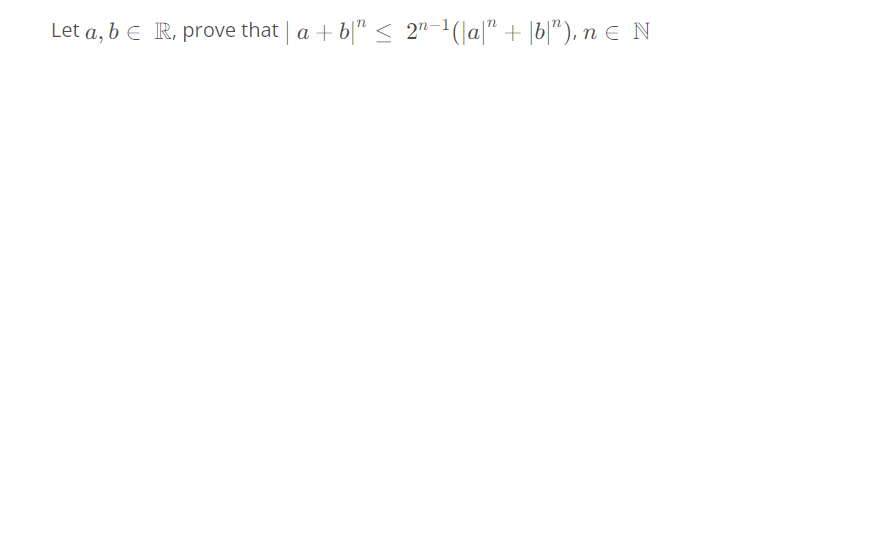
\includegraphics[width=12cm]{exercise4.png}
    \end{figure}
\end{frame}

\begin{frame}
    \frametitle{Mathematical Induction II Exercise}
    Try to write a formal proof !

    \vspace{1em}
    The Fibonacci sequence is defined as follows:
    $$a_1=1$$
    $$a_2=1$$
    $$a_n=a_{n-1}+a_{n-2};n>2$$
    Prove that:
    $$a_n=\frac{(\frac{1+\sqrt{5}}{2})^n-(\frac{1-\sqrt{5}}{2})^n}{\sqrt{5}}$$
\end{frame}

\begin{frame}
    \frametitle{Reference}
    \begin{itemize}
        \item Exercises from 2021--Vv186 TA-Ni Yinchen .
        \item Exercises from 2021--Vv186 TA-Huang Yue .
        \item Learn from 2021--Vv186 TA-Ding Zizhao
        \item Learn from 2021--Vv186 TA-Ma Tianyi
        \item Learn from 2021--Vv186 TA-Sun Meng
    \end{itemize}
\end{frame}

\begin{frame}
    \begin{center}
        {\Huge Thanks $\&$ Have Fun !}
    \end{center}
\end{frame}

\end{document}